\section{Service company}

In service industries, IT plays a dual role: it's both a tool for creating services and a channel for delivering them. 
Unlike in manufacturing, services are typically produced at the same time they are delivered to the customer.

\subsection{Service value chain}
The concept of the value chain, originally introduced by Porter, can also be applied to service businesses. 
However, in services, the boundaries between production and delivery are often blurred.
\begin{figure}[H]
    \centering
    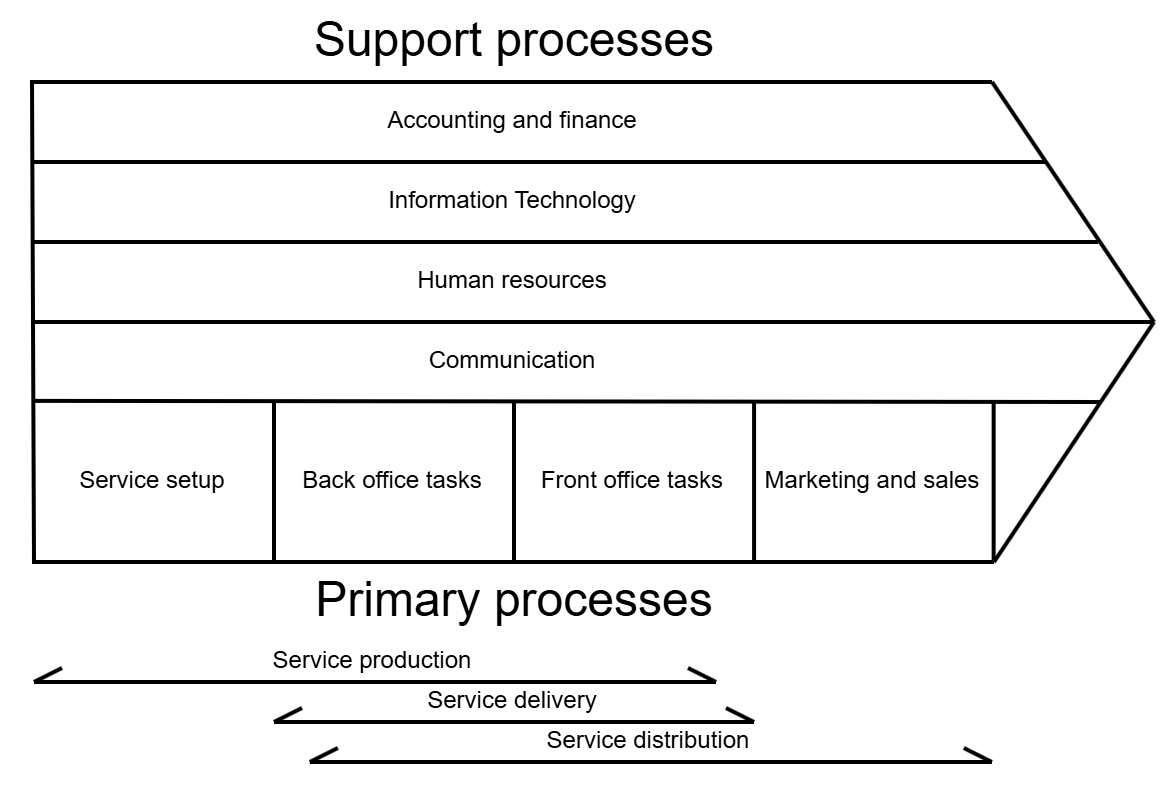
\includegraphics[width=0.75\linewidth]{images/bis13.png}
    \caption{Service value chain}
\end{figure}

\begin{definition}[\textit{Service set-up}]
    Service set-up is the set of tasks required to prepare the company's production capacity.
\end{definition}
\begin{definition}[\textit{Back-office tasks}]
    Back-office tasks are are production tasks carried out without the presence of the customer.
\end{definition}
\begin{definition}[\textit{Front-office tasks}]
    Front-office tasks are tasks involve direct interaction with the customer and are also triggered by a specific customer request.
\end{definition}
\begin{definition}[\textit{Marketing and sales}]
    Marketing and sales are activities focused on promoting the company's services, attracting potential clients, and closing service contracts with new customers.
\end{definition}

\subsection{Inter-functional information processes}
Inter-functional information processes are essential for coordinating production and operations across different functions within a company. 
In service companies, two key processes stand out:
\begin{itemize}
    \item \textit{Order management}: this process handles all the information related to customer orders
        In service companies, order management plays a role similar to operations management in manufacturing firms.
    \item \textit{Knowledge management}: this process deals with collecting and organizing new customer-related information acquired during service production and delivery. 
        The goal is to transform this raw, often unstructured, data into structured knowledge that can be used to improve future services and enhance customer satisfaction. 
        In the context of service companies, knowledge management effectively replaces traditional materials management.
\end{itemize}
\noindent Customizing services to individual customer needs is a key driver of customer satisfaction. 
To do this well, companies need detailed knowledge about each customer.
This knowledge is typically gathered informally during interactions with customers. 
However, this information is often unstructured and difficult to act on directly.
Knowledge management helps by converting these scattered insights into organized, actionable knowledge and linking them to specific service processes.

Knowledge management is not a one-time activity; it's a continuous learning cycle. 
As customer needs evolve and external environments change, companies must adapt their processes accordingly.

The knowledge management process involves three main stages:
\begin{enumerate}
    \item Extracting customer knowledge from employees (often called knowledge workers) based on their direct service experiences.
    \item Transforming that knowledge into structured, usable information, which is then stored in the company's systems. 
    \item Designing or updating procedures that use this information to enable greater service personalization and efficiency.
\end{enumerate}
\noindent This process is far more complex than traditional planning systems like MRP, because it requires insight, interpretation, and innovation. 
That's why knowledge management is considered a hybrid of production planning and service innovation.

\subsection{Information Technology integration}
As in manufacturing, IT integration in service companies follows two main approaches:
\begin{itemize}
    \item \textit{Horizontal integration}: enabled by Personal Computers (PC).
    \item \textit{Vertical integration}: enabled by client-server architectures. 
\end{itemize}

\paragraph*{Personal Computer}
PCs began to gain traction in the 1980s, marking a major shift in how work was done. 
Unlike manufacturing environments where robots automate production, service companies rely heavily on knowledge workers (individuals who create, process, and apply information to deliver services).
PC aren't the equivalent of robots in service production. 
While robots automate tasks, studies on office work have shown that PCs serve more as support tools rather than automation technologies.
This distinction sparked a wave of research into non-hierarchical, decentralized organizations, where individuals use PCs to make independent decisions and contribute more flexibly.
PCs introduced: flexibility, variety and usability. 

\paragraph*{Client-server architectures}
Mainframes and data centers are powerful systems for managing and storing centralized data.
But on their own, they don't empower individual users.
Client-server architectures bridged this gap by connecting personal computers to centralized systems.
This integration allowed knowledge workers not only to access shared data but also to communicate and collaborate across the organization.
With client-server systems, information can flow between knowledge workers and higher management. 
The organization benefits from seamless, integrated management processes that support both autonomy and coordination.

\subsection{Business Process Re-engineering}
\begin{definition}[\textit{Business Process Re-engineering}]
    Business Process Re-engineering (BPR) refers to the transformational changes involved in integrating IT into service companies.
\end{definition}
\noindent While it originated in manufacturing, by the 1990s it was clear that BPR had an even greater impact on the service sector. 
Several trends illustrate how BPR reshaped service delivery:
\begin{itemize}
    \item \textit{Increased delegation}: tasks were pushed downward in the organization, giving more responsibility and autonomy to frontline employees.
    \item \textit{More complex sales roles}: sales staff evolved from simply selling services to guiding customers through service procedures.
    \item \textit{Shift toward customer care}: he focus moved from one-time service sales to long-term customer relationships.
         This required storing detailed customer histories in centralized systems, enabling better support and personalization.
\end{itemize}